% ============================================================
%  sec-4-technical-context.tex  —  1.4 Technical Context
% ============================================================

\section{Technical Context: AI Infrastructure Evolution}
\label{sec:technical-context}

% ── 1.4.1 ────────────────────────────────────────────────────
\subsection{Introduction to AI Infrastructure}
\label{subsec:ai-infra-intro}

AI infrastructure encompasses the integrated hardware, software, and
system-level components that enable the training, deployment, and operation of
artificial intelligence models at scale. Unlike traditional \acrshort{it}
infrastructure optimised for general-purpose data processing, AI infrastructure
is specifically designed for the massive parallel computational demands of
matrix operations, tensor computations, and neural network workloads.

The infrastructure stack is tightly coupled across four abstraction layers:
hardware, system software, AI frameworks, and orchestration platforms.

AI infrastructure has become a strategic pillar for three interconnected
reasons. First, the AI accelerator market is projected to grow from
\$45B in 2024 to \$500B by 2030 (35\% \acrshort{cagr}), reflecting its
economic significance. Second, NVIDIA's 92\% share of the data centre GPU
market has spurred sovereign AI initiatives in the EU, China, and other regions.
Third, AI computing power has been doubling approximately every 6.8 months —
far exceeding Moore's Law — requiring continuous infrastructure innovation.

% ── 1.4.2 ────────────────────────────────────────────────────
\subsection{Evolution of Computing Architectures}
\label{subsec:arch-evolution}

\subsubsection{CPU Era (1940s–2006)}
\label{subsubsec:cpu-era}

From the 1940s through 2006, \acrfull{cpu}s served as the sole computational
backbone for AI research. While their complex control units excel at
general-purpose branching logic, they face fundamental throughput and bandwidth
limitations for modern parallel AI workloads, as summarised in \tabref{cpu-limits}.

\begin{figure}[H]
    \centering
    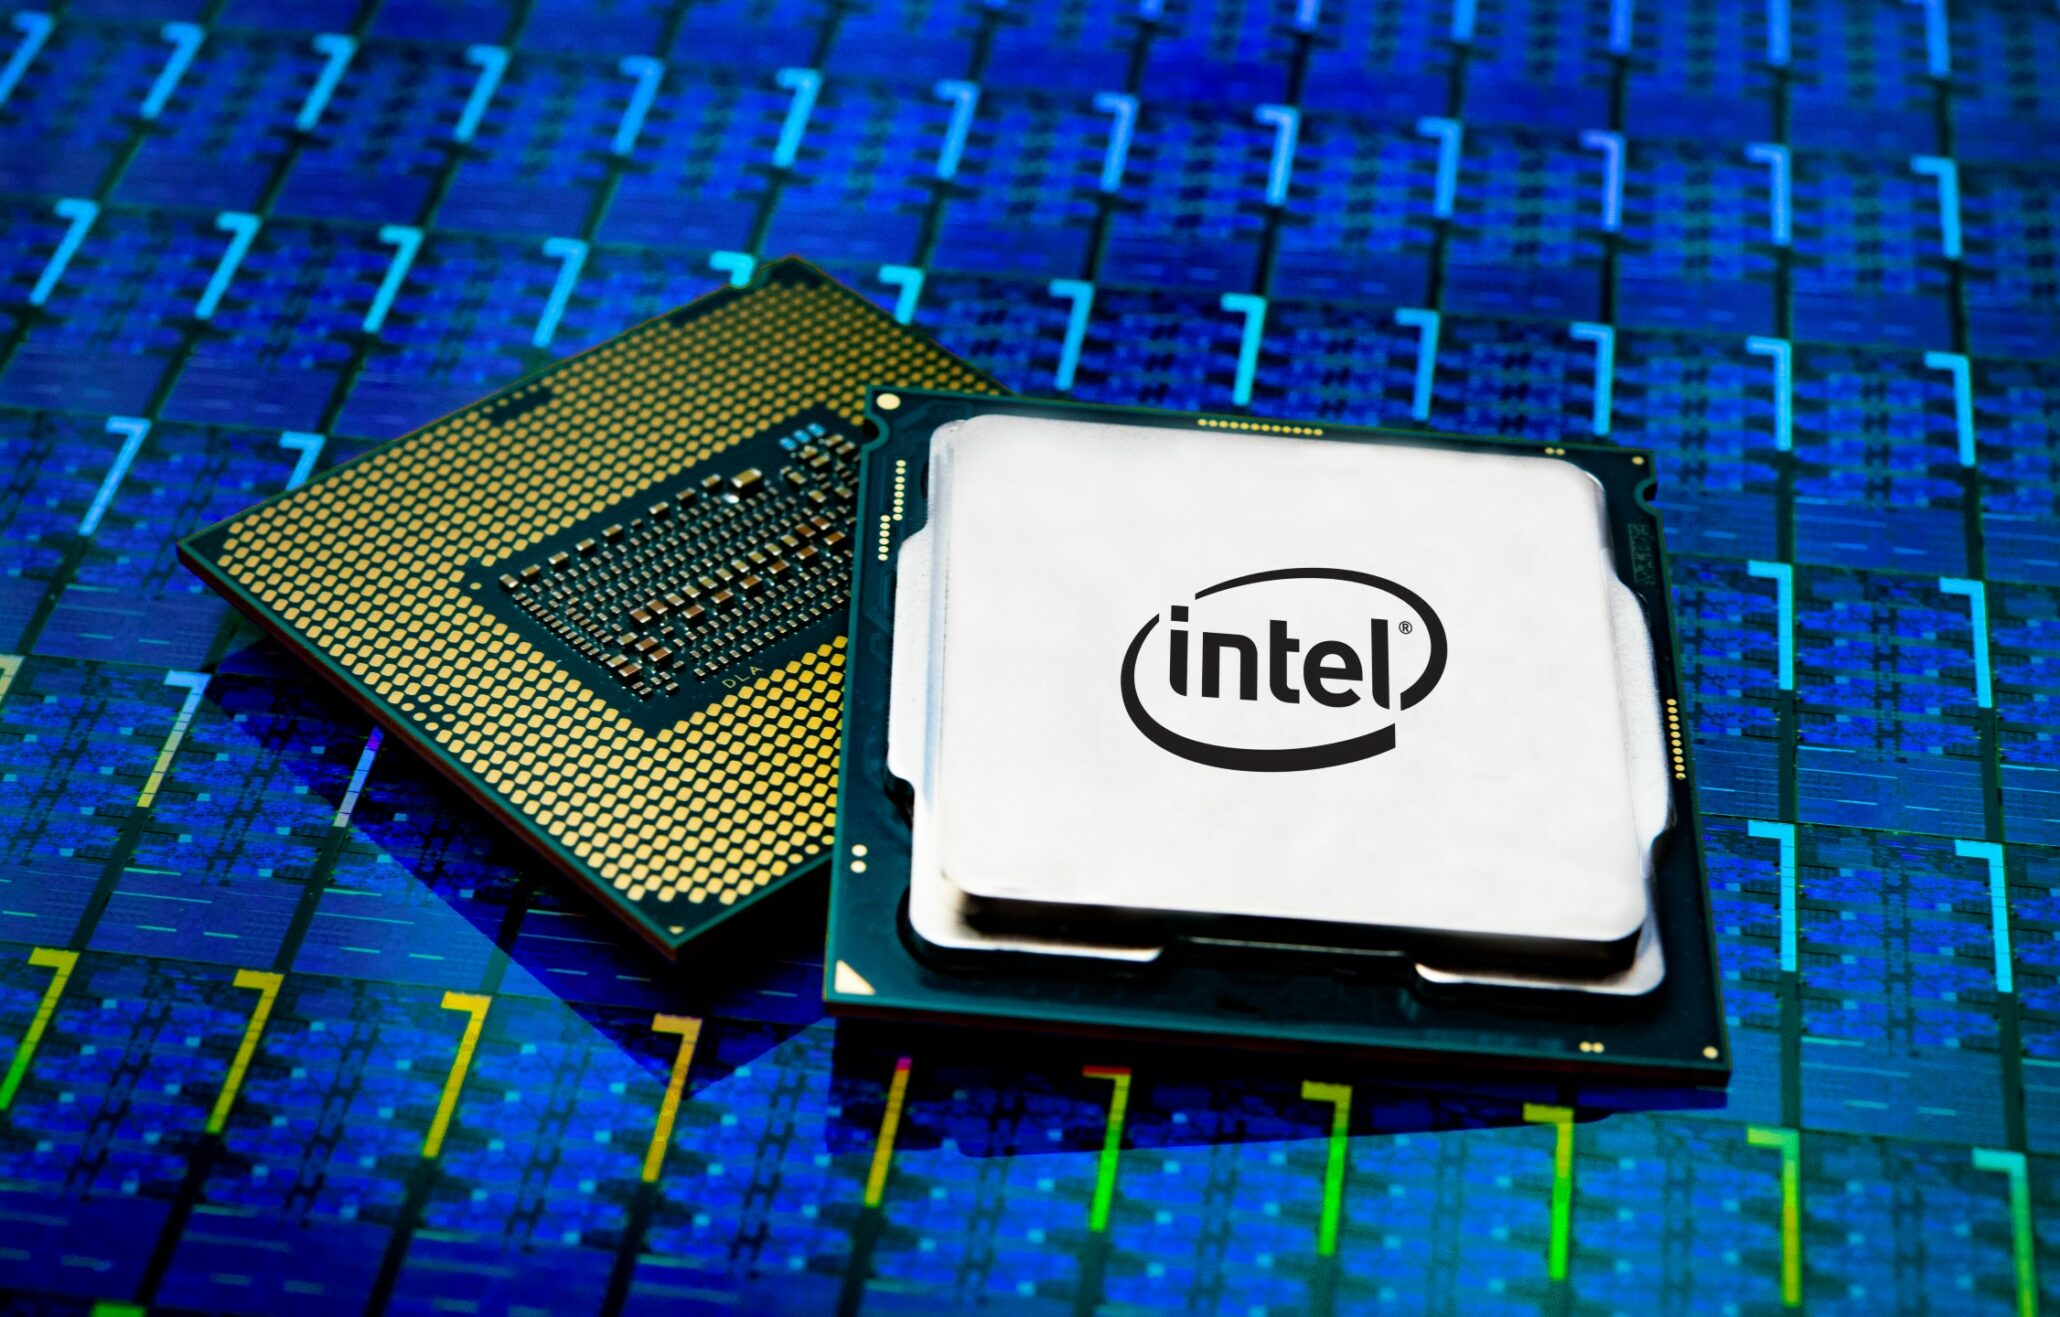
\includegraphics[width=0.5\textwidth]{images/figures/intel-cpu.jpg}
    \caption{Intel CPU Chip}
    \label{fig: Intel CPU Chip}
\end{figure}

\begin{table}[htbp]
  \centering
  \caption{CPU architectural limitations for AI workloads}
  \label{tab:cpu-limits}
  \begin{tabularx}{\textwidth}{lX}
    \toprule
    \tableheader{Limitation & Technical Explanation and AI Impact} \\
    \midrule
    Sequential bottleneck
      & Typical CPUs have 4–96 cores optimised for sequential execution.
        Training ResNet-50 on a CPU takes $\approx$100$\times$ longer than on a GPU. \\
    \rowcolor{TableRowOdd}
    Limited memory bandwidth
      & DDR4/DDR5 bandwidth: 50–200 GB/s — insufficient for large-model
        weight streaming (requires 1–3 TB/s). \\
    Poor FP throughput
      & Single-precision FP32: 0.5–2 TFLOPS; deep learning requires
        tens to hundreds of TFLOPS. \\
    \bottomrule
  \end{tabularx}
\end{table}

\subsubsection{GPU Era (2006–Present)}
\label{subsubsec:gpu-era}

The pivotal transition occurred in 2006 when NVIDIA introduced
\acrfull{cuda}, transforming GPUs from graphics accelerators into
general-purpose parallel processors. The breakthrough moment came in 2012
when AlexNet, trained on GPUs, won ImageNet with 15.3\% top-5 error (vs.\
26.2\% for the best CPU-based approach), demonstrating GPU-accelerated
training 10–100$\times$ faster than CPUs.

Modern data centre GPUs achieve exceptional AI throughput through architectural
features aligned with neural network workloads. The NVIDIA H100, for example,
delivers 989 TFLOPS for FP8 sparse operations with 3,350 GB/s HBM3 memory
bandwidth. The CUDA ecosystem amplified this hardware advantage through a suite
of optimised libraries:

\begin{figure}[H]
    \centering
    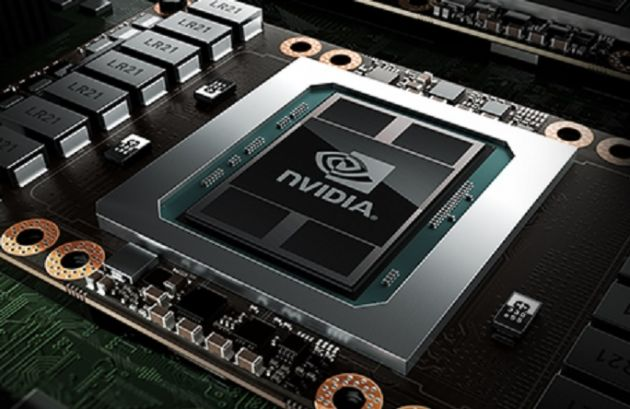
\includegraphics[width=0.5\textwidth]{images/figures/gpu-nvidia.jpg}
    \caption{NVIDIA GPU Chip}
    \label{fig: NVIDIA GPU Chip}
\end{figure}

\begin{table}[htbp]
  \centering
  \caption{Core CUDA ecosystem components and their impact}
  \label{tab:cuda-ecosystem}
  \begin{tabularx}{\textwidth}{llX}
    \toprule
    \tableheader{Component & Function & Performance Impact} \\
    \midrule
    cuDNN     & Deep neural network primitives & 5–10$\times$ speedup for NN operations \\
    \rowcolor{TableRowOdd}
    cuBLAS    & Linear algebra operations       & Foundation for framework optimisations \\
    TensorRT  & Inference optimisation engine   & 3–5$\times$ faster inference \\
    \rowcolor{TableRowOdd}
    NCCL      & Multi-GPU collective communications & Enables distributed training at scale \\
    \bottomrule
  \end{tabularx}
\end{table}

Despite their advantages, GPUs carry inherent limitations: the H100 consumes
700W TDP; training GPT-3 alone required $\approx$1,287 MWh; and a single
DGX H100 system costs \$300,000–\$400,000. Furthermore, approximately 40\%
of GPU transistors are dedicated to graphics features unused in AI workloads.

\subsubsection{Specialised AI Accelerators (NPUs, TPUs, ASICs)}
\label{subsubsec:specialized-accelerators}

Recognising GPU limitations, the industry transitioned toward
Domain-Specific Architectures (\acrshort{dsa}s). Google accelerated this
shift with its Tensor Processing Unit (\acrshort{tpu}) in 2015 — an ASIC
designed exclusively for tensor computations. \tabref{accelerator-comparison}
compares key accelerator specifications.

\begin{figure}[H]
    \centering
    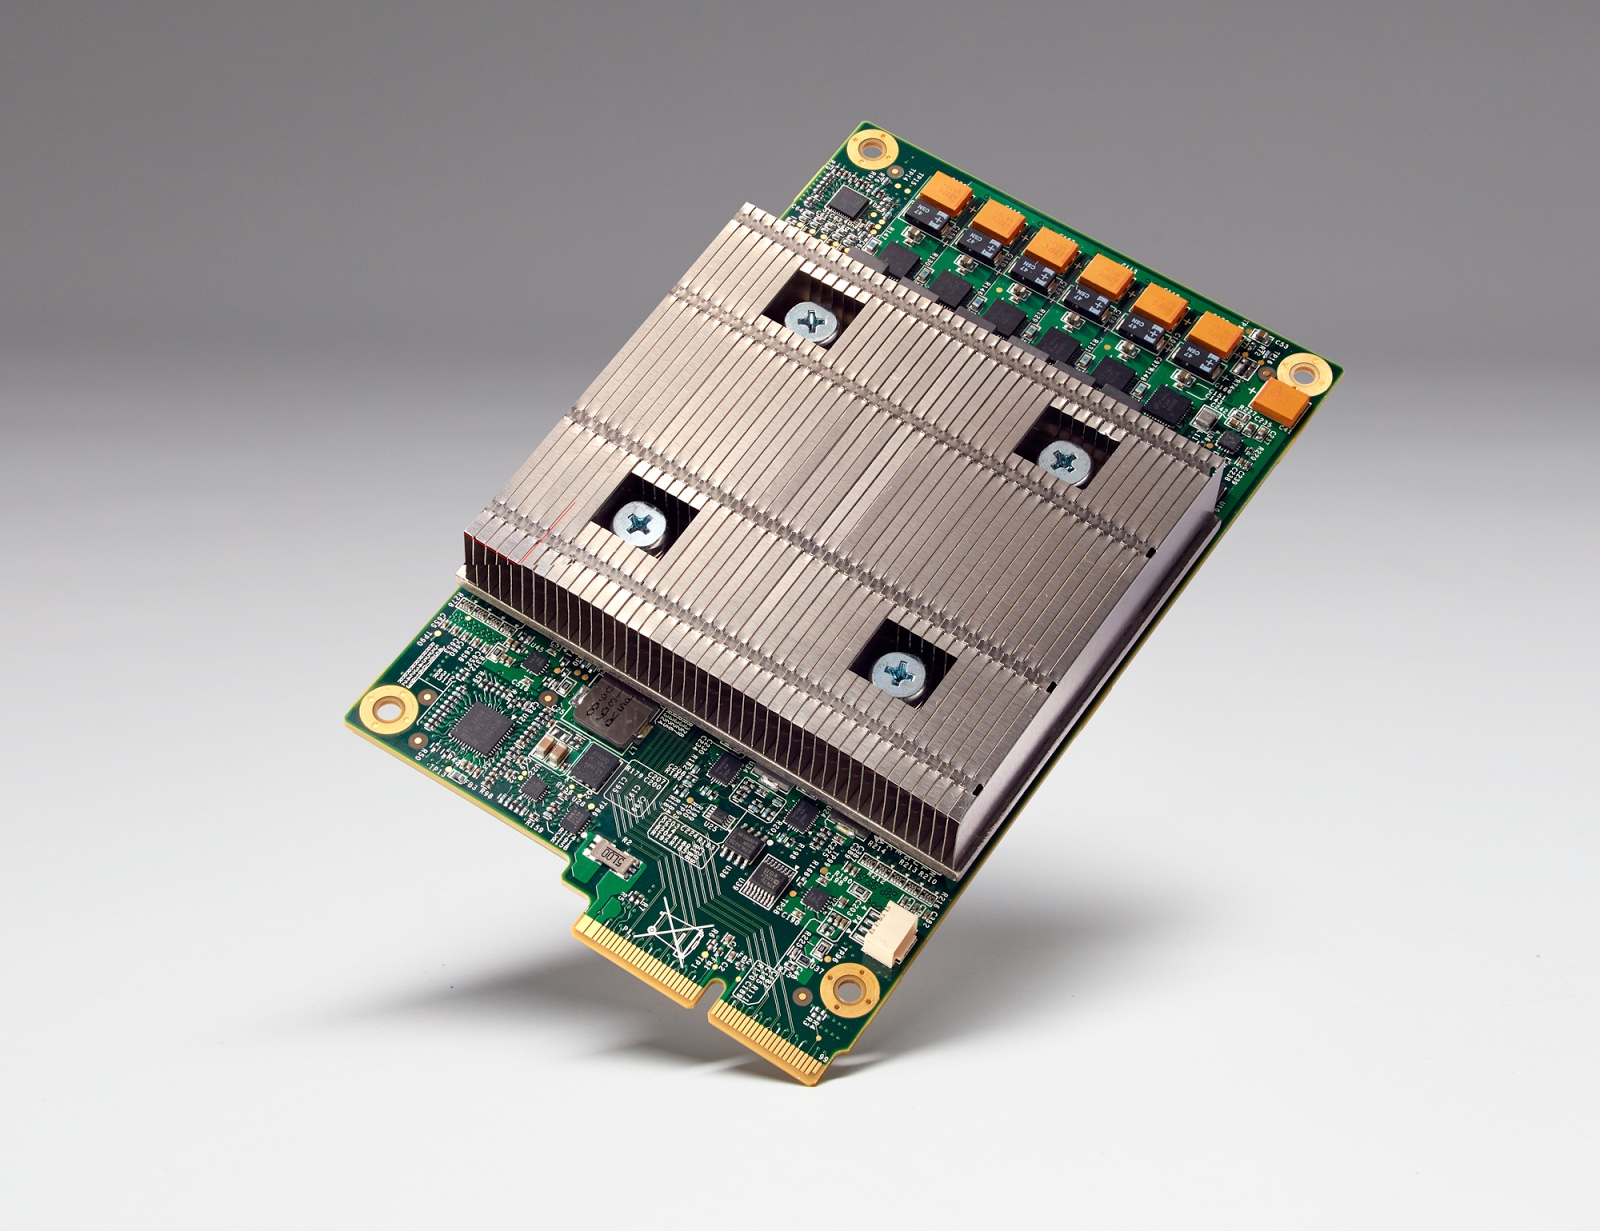
\includegraphics[width=0.5\textwidth]{images/figures/tpu.jpg}
    \caption{Google TPU Chip}
    \label{fig: Google TPU Chip}
\end{figure}

\begin{table}[htbp]
  \centering
  \caption{Comparative specifications: GPU vs. NPU vs. ASIC}
  \label{tab:accelerator-comparison}
  \begin{tabularx}{\textwidth}{lXXX}
    \toprule
    \tableheader{Attribute & GPU (H100) & NPU (Ascend 910B) & ASIC (TPU v4)} \\
    \midrule
    Architecture   & General parallel + graphics & Pure tensor accelerator & Fixed-function \\
    \rowcolor{TableRowOdd}
    Peak FP16      & 989 TFLOPS                 & 256 TFLOPS             & 275 TFLOPS \\
    Memory / BW    & 80 GB HBM3, 3,350 GB/s    & 64 GB HBM2, 1,200 GB/s & 32 GB HBM2 \\
    \rowcolor{TableRowOdd}
    TDP            & 700 W                      & 310 W                  & 170 W \\
    Efficiency     & $\approx$1.5 TOPS/W        & $\approx$3–4 TOPS/W    & $\approx$5 TOPS/W \\
    \rowcolor{TableRowOdd}
    Ecosystem      & CUDA (mature, proprietary) & CANN (Huawei)          & XLA/JAX (Google) \\
    \bottomrule
  \end{tabularx}
\end{table}

% ── 1.4.3 ────────────────────────────────────────────────────
\subsection{Increasing AI Computational Demands}
\label{subsec:compute-demands}

The exponential growth in AI compute demands has been the primary driver
behind the hardware evolution described above. From AlexNet (2012) to GPT-4
(2023), parameter counts increased from 60 million to an estimated 1.7
trillion — a 28,000$\times$ increase. Training compute grew even more
dramatically, from approximately $10^{16}$ FLOPs to beyond $10^{25}$ FLOPs —
a billion-fold increase in just eleven years.

This multiplicative structure means that both model size and data scale
jointly drive training cost. \tabref{model-compute} illustrates the growth trajectory.

\begin{table}[htbp]
  \centering
  \caption{Growth in training compute for landmark models}
  \label{tab:model-compute}
  \begin{tabularx}{\textwidth}{lllll}
    \toprule
    \tableheader{Model & Year & Parameters & Training FLOPs & Dataset} \\
    \midrule
    AlexNet & 2012 & 60M    & $\sim$$10^{16}$ & 1.2M images \\
    \rowcolor{TableRowOdd}
    GPT-2   & 2019 & 1.5B   & $\sim$$10^{21}$ & 40 GB text \\
    GPT-3   & 2020 & 175B   & $3.1 \times 10^{23}$ & 300B tokens \\
    \rowcolor{TableRowOdd}
    PaLM    & 2022 & 540B   & $6.5 \times 10^{24}$ & 780B tokens \\
    GPT-4   & 2023 & $\sim$1.7T & $>$$10^{25}$ & $\sim$13T tokens \\
    \bottomrule
  \end{tabularx}
\end{table}

This growth rate — doubling roughly every 6.8 months — far exceeds historical
Moore's Law (18–24 months per doubling) and creates an energy and cost crisis.
Training GPT-3 consumed $\approx$1,287 MWh and cost $\approx$\$4.6M in cloud
compute; GPT-4 is estimated at \$63–78M. Data centre AI power demand is
projected to more than double by 2030, potentially reaching 94.5 GW globally.

% ── 1.4.4 ────────────────────────────────────────────────────
\subsection{GPU Ecosystem Dominance}
\label{subsec:gpu-dominance}

NVIDIA commands approximately 92\% of the data centre GPU market as of 2024,
a position built on three interlocking advantages: (1) the CUDA software stack
with 4+ million developers and a decade-and-a-half head start; (2) continuous
architectural innovation (Volta $\to$ Turing $\to$ Ampere $\to$ Hopper $\to$
Blackwell); and (3) a mature developer ecosystem where over 95\% of papers at
top AI conferences use NVIDIA hardware, creating reproducibility norms that
reinforce adoption.

\begin{figure}[H]
    \centering
    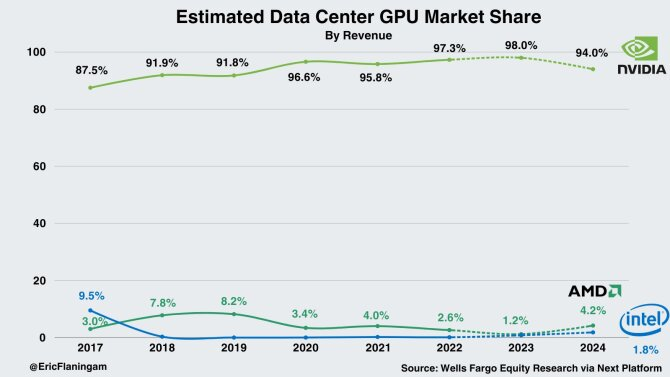
\includegraphics[width=0.7\textwidth]{images/figures/GPU-market-share.jpg}
    \caption{GPU Market Share 2024}
    \label{fig: GPU Market Share 2024}
\end{figure}

This dominance, however, carries systemic risks. CUDA is proprietary and
NVIDIA-exclusive, creating prohibitive migration costs for organisations with
large CUDA codebases. H100 GPUs sell at \$25,000–\$40,000 per unit and carry
36–52 week delivery lead times. Training large models requires
multi-node clusters drawing hundreds of megawatts. Communication overhead can
consume 30–50\% of training time in large clusters without specialised
interconnects. US export restrictions on advanced AI chips to China (2022–2023)
further exposed the fragility of a single-vendor, single-geography ecosystem.

% ── 1.4.5 ────────────────────────────────────────────────────
\subsection{Hardware Specialisation Trends}
\label{subsec:hw-specialisation}

The semiconductor industry is undergoing a fundamental shift from
general-purpose to domain-specific architectures, driven by the convergence
of three constraints: the end of Moore's Law scaling, energy efficiency
boundaries, and the specialised computational patterns of AI workloads.

At process nodes below 5nm, quantum tunnelling effects and manufacturing
complexity make further density increases prohibitively expensive. Meanwhile,
AI workloads exhibit highly regular computational patterns — over 90\%
matrix multiplications and convolutions — that general-purpose processors
cannot exploit efficiently.

\begin{table}[htbp]
  \centering
  \caption{Architectural comparison across computing paradigms}
  \label{tab:arch-comparison}
  \begin{tabularx}{\textwidth}{lXXX}
    \toprule
    \tableheader{Criterion & CPU & GPU & NPU/ASIC} \\
    \midrule
    Parallelism   & Sequential + limited parallel & Thousands of cores  & Systolic arrays, MAC units \\
    \rowcolor{TableRowOdd}
    Precision     & FP32/FP64                    & FP16/FP32           & INT8/FP16 optimised \\
    Power (data centre) & 65–350W               & 300–700W            & 10–310W \\
    \rowcolor{TableRowOdd}
    Efficiency    & $\approx$0.1 TOPS/W          & $\approx$2 TOPS/W   & 5–50+ TOPS/W \\
    Best use case & Control logic, preprocessing & Training, batch inf. & Inference, edge AI \\
    \bottomrule
  \end{tabularx}
\end{table}

The AI computing landscape is bifurcating into cloud (training and large-scale
batch inference) and edge (real-time, low-latency inference) domains, each with
distinct hardware requirements.

% ── 1.4.6 ────────────────────────────────────────────────────
\subsection{Rise of Neural Processing Units}
\label{subsec:npu-rise}

A Neural Processing Unit is a specialised microprocessor explicitly designed
to accelerate AI and machine learning workloads by implementing the
mathematical structure of neural networks directly in silicon. NPUs incorporate
thousands of multiply-accumulate (\acrshort{mac}) units arranged in systolic
array patterns, enabling massive parallel matrix multiplication — the
fundamental operation in deep learning.


